\chapter{Business Intelligence Workload}
\label{sec:bi}

The Business Intelligence (BI) workload is the SNB's analytical (OLAP) workload.
As such, it defines complex read queries that touch a significant portion of the data (see \autoref{sec:bi-reads}).
Additionally, it defines daily batches of updates over a 33-day period
(see
\autoref{sec:bi-insert-operations} for inserts and
\autoref{sec:bi-delete-operations} for deletes).
% The available batches are
% 2012-11-29,
% 2012-11-30,
% 2012-12-01, \ldots
% 2012-12-31;
% yielding 33~batches in total.

\subsection*{Related Publications}

The BI workload was published in PVLDB 2022~\cite{DBLP:journals/pvldb/SzarnyasWSSBWZB22}.

\subsection*{Related Software Components}

\begin{itemize}
    \item Datagen (Spark-based): \url{https://github.com/ldbc/ldbc_snb_datagen_spark}
    \item Driver and reference implementations: \url{https://github.com/ldbc/ldbc_snb_bi}
\end{itemize}

%%%%%%%%%%%%%%%%%%%%%%%%%%%%%%%%%%%%%%%%%%%%%%%%%%%%%%%%%%%%%%%%%%%%%%%%%%%%%%
%%%%%%%%%%%%%%%%%%%%%%%%%%%%%%%%%%%%%%%%%%%%%%%%%%%%%%%%%%%%%%%%%%%%%%%%%%%%%%
%%%%%%%%%%%%%%%%%%%%%%%%%%%%%%%%%%%%%%%%%%%%%%%%%%%%%%%%%%%%%%%%%%%%%%%%%%%%%%

\section{Overview}
\label{sec:bi-benchmark-overview}

\begin{figure}[htb]
    \centering
    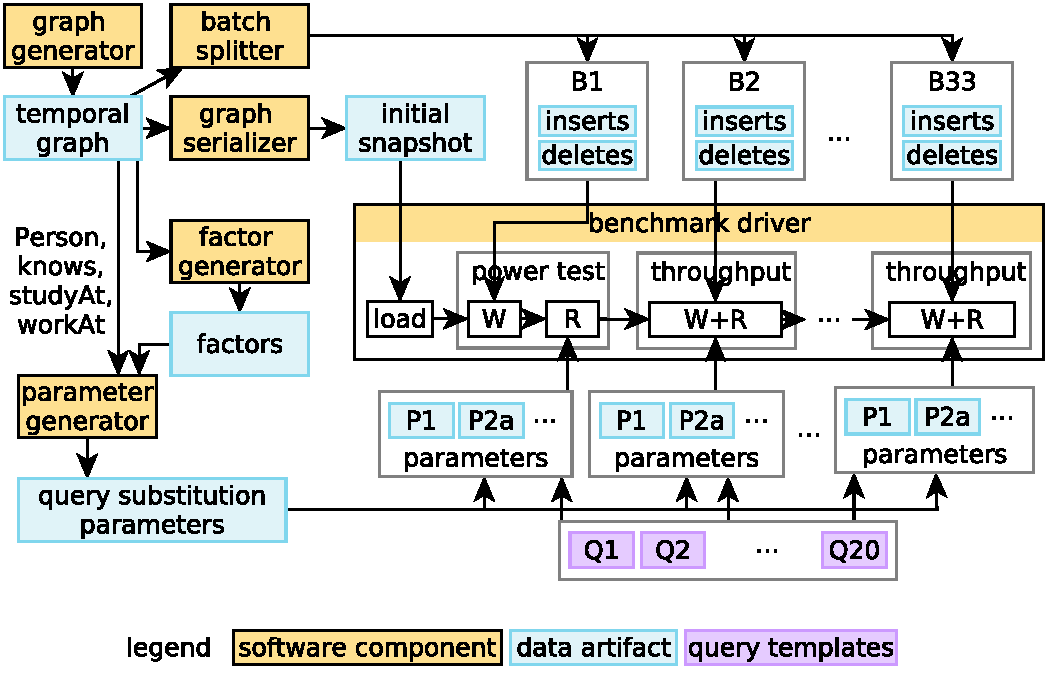
\includegraphics[scale=\yedscale]{figures/bi-workflow}
    \caption{Main software components and data artifacts of the benchmark and their connection to the workflow executed by the BI benchmark driver.}
    \label{fig:bi-workflow}
\end{figure}

An overview of the BI workload is shown in \autoref{fig:bi-workflow}.
The rules for auditing workload implementations are given in \autoref{sec:auditing-bi-workload-audit}.

%%%%%%%%%%%%%%%%%%%%%%%%%%%%%%%%%%%%%%%%%%%%%%%%%%
\section{Read Query Templates}
\label{sec:queries}
%%%%%%%%%%%%%%%%%%%%%%%%%%%%%%%%%%%%%%%%%%%%%%%%%%

%This section discusses the queries (bottom middle part \autoref{fig:benchmark-components}).

\snbbi consists of 20~parameterized \emph{read query templates}, referred to as \emph{queries}. These search for graph patterns (often implying join-heavy operations on many-to-many edges), traverse hierarchies, and compute cheapest paths (\aka weighted shortest paths).
Additionally, they include filtering, grouping, aggregation, and sorting operators.
While all queries explore a large portion of the graph, they only return the top-$k$ (typically 20 or 100) results,
keeping their result sizes compact to avoid emphasizing the client-server network protocol's role in the benchmark~\cite{DBLP:journals/pvldb/RaasveldtM17}.

%------------------------------------------------------------------------------
\subsection{Choke Point-Based Design Methodology}
%------------------------------------------------------------------------------

LDBC's query design process relies on the use of \emph{choke points} (\autoref{sec:choke-points}),
\ie challenging aspects of query processing.
\snbbi includes 38~choke points divided into 9~categories:
aggregation performance,
join performance,
data access locality,
expression calculation,
correlated subqueries,
parallelism and concurrency,
graph specifics,
language features,
and
update operations.
Their coverage is shown in \autoref{tab:query_choke_point}.
In the following, we discuss two challenges that are particularly prevalent in graph workloads.

\subsubsection{Explosive and redundant multi-joins}
In recent years it has become clear that graph pattern matching, or equivalent multi-join queries over many-to-many relationships, typically generate very large intermediate results when executed with traditional join algorithms. This is especially the case for cyclical join graphs (corresponding to cyclic graph queries). % citation for cyclical join graphs?
It was proven in theory~\cite{DBLP:journals/sigmod/NgoRR13} and shown in practice~\cite{DBLP:journals/corr/abs-1210-0481,DBLP:journals/pvldb/MhedhbiS19,DBLP:journals/pvldb/FreitagBSKN20} that ``worst-case optimal'' {\em multi-}join algorithms can avoid these large intermediates and outperform traditional joins. Following this, there has been increased attention on {\em redundancy} in join results (even when produced by worst-case optimal joins), which can be eliminated using {\em factorized} query processing techniques~\cite{DBLP:journals/pvldb/BakibayevOZ12,DBLP:journals/sigmod/OlteanuS16,DBLP:journals/pvldb/GuptaMS21}.
Graph pattern matching queries that contain large join patterns will trigger these phenomena.

\subsubsection{Expressive path finding}
\snbbi contains queries that require an efficient implementation of shortest path finding between many pairs.
Expressing such queries requires a query language which supports either path finding or recursion. The underlying system implementation must then handle this with an optimized execution strategy, as recursing to try all paths will not scale.
As some of this path finding includes on-the-fly computed edges (joins) between nodes, the queries can benefit from {\em path expressions}, as proposed in Oracle's PGQL language~\cite{DBLP:conf/grades/RestHKMC16} and as part of the upcoming GQL and SQL/PGQ languages~\cite{DBLP:conf/sigmod/DeutschFGHLLLMM22}.
The path finding required by \snbbi not only tests connectivity (as supported in SPARQL), but also requires returning the {\em cheapest cost} along weighted paths (necessitating SPARQL extensions~\cite{DBLP:conf/bigdataconf/MizellMR14}).

%------------------------------------------------------------------------------
\subsection{Analysis of Selected Queries}
\label{sec:example-queries}
%------------------------------------------------------------------------------

In order to defeat trivializing complex query performance by query caching, benchmarks can use both frequent updates (which require invalidating caches or maintaining cached intermediates) as well as parameterized query templates.
The BI workload features update batches, so parametrized \emph{read query templates} are necessary to guard against this between the batches.
In this section, we analyze four read query templates.

\emph{Notation:}
We denote the query parameters with the \param{}~symbol and discuss their generation in \autoref{sec:paramgen}.

% #############################################################################
\subsubsection{Q11: Friend triangles}
% #############################################################################

\queryRefCard{bi-read-11}{BI}{11} imposes two key difficulties.
First, systems should efficiently filter the \tKnows edges based on the location of their endpoint \tPersons (\tCountry \param{country}) and the date range.
Second, given a large number of \tKnows edges even after filtering,
efficient enumeration of \texttt{personA}--\texttt{personB}--\texttt{personC} triangles (a cyclic subgraph query)
requires worst-case optimal multi-joins.

% #############################################################################
\subsubsection{Q14: International dialog}
% #############################################################################

\queryRefCard{bi-read-14}{BI}{14} imposes different challenges depending on whether
\tCountries \param{country1} and \param{country2} are correlated or anti-correlated
(\autoref{sec:paramgen-correlations}).
For the ranking, \emph{top-k pushdown} can be exploited:
once a result for a \tCity in \param{country1} is obtained,
extra restrictions in a selection can be added based on the value of this element.
As the score of two \tPersons does not depend on any query parameters,
precomputing and maintaining it as an attribute on the \tKnows edge can be beneficial.

% #############################################################################
\subsubsection{Q18: Friend recommendation}
% #############################################################################

\queryRefCard{bi-read-18}{BI}{18} is inspired by Twitter's recommendation algorithm~\cite{DBLP:conf/www/GuptaGLSWZ13}.
Implementations of this query can exploit factorization:
systems can count the number of mutual friends without explicitly enumerating all
\textsf{<}\texttt{person1}, \texttt{personM}, \texttt{person2}\textsf{>} tuples.

% #############################################################################
\subsubsection{Q20: Recruitment}
% #############################################################################

\queryRefCard{bi-read-20}{BI}{20} performs \emph{graph projection}~\cite{DBLP:conf/sigmod/AnglesABBFGLPPS18}.
Instead of materializing this graph in the database,
systems may represent it using a compact in-memory structure such as CSR (Compressed Sparse Row)~\cite{DBLP:books/daglib/0009092}.
To perform the cheapest path computation, a single-source shortest path algorithm
(starting from \param{person2}), such as Dijkstra's algorithm, can be used.
As the projected graph %(incl. its edge weights)
is independent of query parameters, precomputing and maintaining it can be beneficial.



%%%%%%%%%%%%%%%%%%%%%%%%%%%%%%%%%%%%%%%%%%%%%%%%%%
\section{Parameter Curation for BI Queries}
\label{sec:paramgen}
%%%%%%%%%%%%%%%%%%%%%%%%%%%%%%%%%%%%%%%%%%%%%%%%%%

\subsection{The Need for Parameter Curation}

A disadvantage of executing the same read query template with different parameters is that the intermediate results and runtimes can be severely influenced by the parameter values.
This is particularly the case in \snbbi with its explosive joins, skewed out-degrees, skewed value distributions, correlated value distributions, and structural correlations.
Moreover, the updates (including cascading deletes) can significantly change the portion of the graph reached by the same query executed at different times. % logical times? stages?
In order to keep query performance understandable we need to actively {\em curate} parameters, such that different parameters executed at different logical times %in different batches
still lead to stable and, therefore, understandable results.
We achieve this through \emph{parameter curation}~\cite{DBLP:conf/tpctc/GubichevB14,DBLP:conf/sigmod/ErlingALCGPPB15}, a data mining process of looking for parameter values with suitably similar characteristics.

\subsection{Parameter Generation Steps}
\label{sec:parameter-curation-method}

Our parameter curation process is a two-step process:
we first generate \emph{factors} followed by the \emph{parameters} (\autoref{fig:bi-workflow}).
These components are executed for each scale factor and are independent of the serialization format/layout of the data set.

\subsubsection{Factor Generator}
The factor generator produces 21~\emph{factor tables} containing summary statistics from the temporal graph,
\eg
the number of \tPersons per \tCity
or
the number of \tMessages per day for each \tTag.


\subsubsection{Parameter Generation}
\label{sec:parameter-generation-query}

To find suitable substitution parameters that (presumably) lead to the same amount of data access and thus similar runtimes,
we first identify the factor table containing the summary statistics of the query's parameters.
For example, Q14's template uses the parameters \tCountry \param{country1} and \tCountry \param{country2}.
Therefore, we use the \texttt{countryPairsNumFriends} factor table which contains \param{country1}, \param{country2} pairs and the number of friendships on \tPerson lives in \param{country1} and the other lives in \param{country2}.
Using this table, we select the $p$th percentile from the distribution as the \emph{anchor},
then rank the rest of the distribution based on their absolute difference from the anchor and take the top-$k$ values.
We shuffle the values using a hash function to avoid introducing artificial locality, where \eg subsequent queries start in nodes from the same ID range.
\autoref{lst:q14-parameter-generation} shows the SQL query implementing the parameter generation for Q14\variantA.

\subsection{Parameter Curation for Graph Queries}

We discuss two parameter curation cases that are particularly important in graph data management.

\subsubsection{Correlated \vs Anti-Correlated Parameters}
\label{sec:paramgen-correlations}

Our parameter curation provides a straightforward way of selecting start entities which
are affected by (structural or attribute-level) correlation \vs anti-correlation:
corresponding parameters can be found by selecting a high \vs low percentile as the anchor
in the parameter generation query.
For example, for Q14 (\autoref{sec:bi-read-14}),
we selected
variant~\variantA to $p=0.98$ (correlated) and
variant~\variantB to $p=0.03$ (anti-correlated).

\subsubsection{Path Queries}
\label{sec:path-queries}

\snbbi queries Q15, Q19, Q20 include cheapest path finding queries computed between given (sets of) \tPersons.
These queries are particularly challenging for parameter curation:
if there is no path between the two endpoints, query runtimes are significantly higher as the search has to traverse an entire connected component to ensure that no path exists.
Moreover, the presence of a path between two nodes \emph{at a given time} does not guarantee that it will always exist during the benchmark execution as deletions can render the endpoints of a path unreachable.

\subsection{Query Variants}
\label{sec:bi-query-variants}

12~queries have a single variant, while 8~queries have two variants, yielding a total of 28~query variants.
As a rule of thumb, variants \variantA are expected to produce a longer runtime
while variants \variantB are expected to be simpler.
Variants of Q2, Q8, Q16 are parametrized with a flashmob \vs a non-flashmob date.
Variants of Q14 and Q19 select correlated \vs non-correlated \tCountries/\tCities.
Q10's variants differ in degree (a start \tPerson with an average number of friends \vs only a few friends), while
Q15's variants have different path lengths and time intervals (4 hops and one week \vs 2 hops and one month).
Q20\variantA selects endpoints where it is guaranteed that \emph{no path exists}, while Q20\variantB selects ones where there is guaranteed that a path exists.

\subsection{Scalability and Reproducibility}
\label{sec:paramgen-scalability}

%Ensuring the parameter generator's scalability and reproducibility relies on the SNB Datagen providing the same characteristics (\autoref{sec:datagen-reproducibility}).

\subsubsection{Scalability}
The \emph{factor generator} is part of the SNB Datagen and runs after the \textit{temporal graph} has been created.
It is implemented in Spark for distributed execution.
While its computations use expensive, aggregration-heavy queries, the derived factor tables are \emph{compact}, \eg SF\numprint{10000} has only 20~GiB of factors in compressed Parquet format, the equivalent of approximately 100~GiB in CSV format, \ie 1\% of the total data set size.
The \emph{parameter generator} queries are executed in DuckDB~\cite{DBLP:conf/sigmod/RaasveldtM19},
which supports vertical scalability and is capable of running the parameter generation for SF\numprint{10000} using less than 512~GiB memory.

\lstset{language=sql,morekeywords={WITHIN}}
\begin{lstlisting}[label=lst:q14-parameter-generation,caption=Parameter generation SQL query for Q14\variantA.]
SELECT country1, country2
FROM (
  SELECT
    country1,
    country2,
    abs(frequency - (
      SELECT percentile_disc(0.98) WITHIN GROUP (ORDER BY frequency) AS anchor FROM countryPairsNumFriends
    )) AS diff
  FROM countryPairsNumFriends
  ORDER BY diff, country1, country2
)
ORDER BY md5(concat(country1, country2))
LIMIT 50
\end{lstlisting}


\subsubsection{Reproducibility}
It is important to guarantee that the parameter curation process is reproducible.
To this end, we leverage that the Datagen and, consequently, the factor generator are reproducible.
To ensure that the parameter generation queries yield deterministic results we define a total ordering in each query.
To provide deterministic shuffling we base the ordering on MD5 hashes (instead of the actual attribute values), see \autoref{lst:q14-parameter-generation}.

%%%%%%%%%%%%%%%%%%%%%%%%%%%%%%%%%%%%%%%%%%%%%%%%%%%%%%%%%%%%%%%%%%%%%%%%%%%%%%
%%%%%%%%%%%%%%%%%%%%%%%%%%%%%%%%%%%%%%%%%%%%%%%%%%%%%%%%%%%%%%%%%%%%%%%%%%%%%%
%%%%%%%%%%%%%%%%%%%%%%%%%%%%%%%%%%%%%%%%%%%%%%%%%%%%%%%%%%%%%%%%%%%%%%%%%%%%%%

\section{Reads}
\label{sec:bi-reads}

\input{query-cards/bi-read-01}
\input{query-cards/bi-read-03}
\input{query-cards/bi-read-04}
\input{query-cards/bi-read-05}
\input{query-cards/bi-read-06}
\input{query-cards/bi-read-07}
\input{query-cards/bi-read-08}
\input{query-cards/bi-read-10}
\input{query-cards/bi-read-14}
\input{query-cards/bi-read-16}
\input{query-cards/bi-read-17}
\input{query-cards/bi-read-18}
\input{query-cards/bi-read-21}
\input{query-cards/bi-read-22}
\input{query-cards/bi-read-25}

% reset counter to make sure the last query card isn't stuck in highlighted mode
\renewcommand{\currentQueryCard}{0}


%%%%%%%%%%%%%%%%%%%%%%%%%%%%%%%%%%%%%%%%%%%%%%%%%%%%%%%%%%%%%%%%%%%%%%%%%%%%%%
%%%%%%%%%%%%%%%%%%%%%%%%%%%%%%%%%%%%%%%%%%%%%%%%%%%%%%%%%%%%%%%%%%%%%%%%%%%%%%
%%%%%%%%%%%%%%%%%%%%%%%%%%%%%%%%%%%%%%%%%%%%%%%%%%%%%%%%%%%%%%%%%%%%%%%%%%%%%%

\section{Insert Operations}
\label{sec:bi-insert-operations}

Insert operations consist of individual inserts for each entity type.
Implementations typically use the same format as the one for loading the initial snapshot of the data set.

%%%%%%%%%%%%%%%%%%%%%%%%%%%%%%%%%%%%%%%%%%%%%%%%%%%%%%%%%%%%%%%%%%%%%%%%%%%%%%
%%%%%%%%%%%%%%%%%%%%%%%%%%%%%%%%%%%%%%%%%%%%%%%%%%%%%%%%%%%%%%%%%%%%%%%%%%%%%%
%%%%%%%%%%%%%%%%%%%%%%%%%%%%%%%%%%%%%%%%%%%%%%%%%%%%%%%%%%%%%%%%%%%%%%%%%%%%%%

\section{Delete Operations}
\label{sec:bi-delete-operations}

\iftoggle{StandaloneWorkloadSpecification}{
    \input{query-cards/delete-01}
\input{query-cards/delete-02}
\input{query-cards/delete-03}
\input{query-cards/delete-04}
\input{query-cards/delete-05}
\input{query-cards/delete-06}
\input{query-cards/delete-07}
\input{query-cards/delete-08}

}{
    See \autoref{sec:delete-operations}.
}
